\documentclass{article}

\usepackage{url}
\usepackage{xspace}
\usepackage{graphicx}
\usepackage{booktabs}
\usepackage{subfigure}
\usepackage{verbatim}
\usepackage{hyperref}
\usepackage{color}

\usepackage{amsmath, amsthm, amssymb}
\usepackage{latexsym}
\usepackage{amsopn}

\newcommand{\moise}{{$\mathcal{M}$\textsc{oise}}\xspace}
\newcommand{\moisem}{{$\mathcal{M}$\textsc{oise}$^{+}$}\xspace}
\newcommand{\aanda}{\textsf{A\&A}\xspace}
\newcommand{\oramas}{\textsf{ORA4MAS}\xspace}
\newcommand{\cartago}{\textsf{CArtAgO}\xspace}
\newcommand{\Jason}{\textit{Jason}\xspace}
\newcommand{\role}[1]{\textit{#1}}
\newcommand{\goal}[1]{{\textsf{#1}}}
\newcommand{\todo}[1]{\textcolor{red}{TODO: }\textcolor{blue}{#1}}
\newcommand{\eqdef}{\ \stackrel{\mathtt{def}}{=} \ }     %definitional equation
\newcommand{\st}{\mid}
\newcommand{\set}[1]{\mathcal{#1}}
\newcommand{\subrole}{\sqsubset}
\newcommand{\normid}[1]{\texttt{\small #1}}
\newcommand{\andalso}{\quad\quad}
\newcommand{\code}[1]{\texttt{#1}}

\newcommand{\pathwp}{../../examples/writePaper}

\newenvironment{rwrule}[2]
{\begin{quote}\ttfamily\begin{tabbing}~~~\=$\leftarrow$ \= ~~~ \= \kill
     \ensuremath{#2}\\
     \rule[2pt]{6.5cm}{.3pt} \hfill \rwlabel{#1}\\}
{\end{tabbing}\end{quote}}
\newcommand{\rwlabel}[1]{{\scshape\itshape\textrm{#1}}}

\theoremstyle{definition} \newtheorem{definition}{Definition}

\sloppy
\setlength\parindent{0pt}
\setlength\parskip{6pt}
\setlength\itemsep{0pt}

\begin{document}

\title{\moise specifications \\ --- draft ---}
\author{Jomi F. H\"ubner}
%\date{April 2010}
\maketitle

\begin{abstract}
  This document presents \moise specifications for ($i$) the
  organisational \emph{model} (OS, OE), and ($ii$) the
  \emph{semantics} in terms of translation to NOPL. The focus is on
  the formalisation, no motivations, examples, or detailed
  explanations are thus provided (these aspects are considered in the
  papers listed in the end of this document).

  The current implementation of \moise (release 0.7) is considered in
  this document and not the variants/experiments/extensions
  published in some papers.
\end{abstract}


\newpage
\tableofcontents
\newpage


\section{Organisation Model}

The \moise organisation model started on paper \cite{hannoun:02} and
then was extended in \cite{hubner:02b} and \cite{gateau:eumas05}. This
section is thus based on these papers. Although, as stated in the
abstract, this document considers the implemented version of the
model, as available in \url{http://moise.sourceforge.net}.

Sets, relations, and functions are used to define the elements that
compose the organisational model of \moise. The informal meaning of
these elements are presented in the papers cited above. The formal
meaning is defined in Sec.~\ref{sec:sem}.

\todo{use Z notation}

\subsection{Organisational Specification}


\begin{definition}[Organisational Specification]
  An Organisational Specification (OS) is defined by its three
  dimensions: structural, functional, and normative.
  \begin{displaymath}
    \langle id, SS, FS, \set{NS} \rangle
  \end{displaymath}
  where
  \begin{itemize}
  \item $id$ is a unique identification of the OS;
  \item $SS : \set{SS}$ is a structural specification ($\set{SS}$ is
    the set of all SSs and the \emph{type} of $SS$);
  \item $FS : \set{FS}$ is a functional specification ($\set{FS}$ is
    the set of all FSs); and
  \item $\set{NS}$ is a set of norms.
  \end{itemize}
\end{definition}

\subsubsection{Structural Specification}


\begin{definition}[Structural Specification]
  A Structural Specification (SS) is defined by the
  elements of the following tuple:
  \begin{displaymath}
    \langle \set{R}, \sqsubset, rg, \set{L} \rangle
  \end{displaymath}
  where
  \begin{itemize}
  \item $\set{R}$ is a set of identifiers of roles of the organisation;
  \item $\sqsubset \; : \set{R} \times \set{R}$ is an inheritance
    relation among roles;\footnote{$\rho \subrole q$ means $q$ is a
      sub-role of $\rho$ or $\rho$ is a super-role of $q$.}
  \item $rg : \set{GS}$ is the specification of the root group of
    the organisation ($\set{GS}$ is the set of all group
    specifications and the type of $rg$);
  \item $\set{L}$ is a set of links between roles in the scope of
    the group being defined.
  \end{itemize}
Inheritance properties:
\begin{itemize}
\item Anti-symmetric
  \begin{equation}
  \rho \subrole \rho' \land \rho' \subrole \rho   \Rightarrow \rho = \rho'
 \end{equation}

\item Transitivity
  \begin{equation}
    \rho \subrole \rho' \land \rho' \subrole \rho'' \Rightarrow \rho \subrole \rho''
  \end{equation}

\item Role hierarchy root ($\rho_{soc}$)
  \begin{eqnarray}
    &&\rho_{soc} \in \mathcal{R}\\
    &&\forall \rho \in (\mathcal{R} \backslash \{\rho_{soc}\}) \st {\rho_{soc} \subrole \rho}\\
    &&\nexists \rho \in \mathcal{R} \st \rho \subrole \rho_{soc}
  \end{eqnarray}

\end{itemize}
\end{definition}

\begin{definition}[Link]
  A link is defined by a tuple:
  \begin{displaymath}
    \langle s, t, k, p \rangle
  \end{displaymath}
  where
  \begin{itemize}
  \item $s : \set{R}$ is the role source of the link;
  \item $t : \set{R}$ is the role target of the link;
  \item $k : \{ acq, com, auth\}$ is the type the link
    (acquaintance, communication, or authority).
  \item $p : \{ intra, inter \}$ is the scope of the link
    (inter-group or intra-group).
  \end{itemize}

  Reads: an agent playing the role $s$ has the link of type $k$ to
  agents playing role $t$ in scope $p$.

  Properties:
  \begin{itemize}
  \item Authority implies communication
    \begin{equation}
       \langle s, t, auth, p \rangle \Rightarrow  \langle s, t, com, p \rangle
    \end{equation}

  \item Communication implies acquaintance
    \begin{equation}
       \langle s, t, com, p \rangle \Rightarrow  \langle s, t, acq, p \rangle
    \end{equation}

  \item Inheritance (all links defined for a role is inherited by its sub-roles)
    \begin{eqnarray}
    \langle s, t, k, p \rangle \in \set{L} \land s \subrole s' &\Rightarrow&  \langle s', t, k, p \rangle \in \set{L}\\
    \langle s, t, k, p \rangle \in \set{L} \land t \subrole t' &\Rightarrow&  \langle s, t', k, p \rangle  \in \set{L}
    \end{eqnarray}

  \end{itemize}
\end{definition}

The scope $intra$ means that the link is valid only inside a group
instance: an agent playing the role $s$ in an instance group $g$ has
the link to agents playing the role $t$ in the same group $g$. The
scope $inter$ means that the link exists only for different group
instances: an agent playing the role $s$ in an instance group $g$ has
the link to agents playing the role $t$ in the another group $g'$,
where $g \neq g'$. In the case where both scopes are defined, the link
exists despite the instances of the groups.

\begin{definition}[Group Specification]
  A Group Specification (GS) is defined by the elements of the following tuple:
  \begin{displaymath}
    \langle id, compat, maxrp, minrp, maxsg, minsg \rangle
  \end{displaymath}
  where
  \begin{itemize}
  \item $id$ is a unique identification of the GS;
  %\item $\set{R}_{gs} \subseteq \set{R}$) is a set of
  %  identifiers of roles that can be played in the group;
 \item $compat : \set{R} \to 2^{\mathcal{R}}$ is a
    function that maps each role to the set of its compatible roles;
  \item $maxrp : \mathcal{R} \to \mathbb{Z}$: is a function that maps
    each role to the maximum number of players of that role in the
    group (upper bound of role cardinality);\footnote{If role $\rho$
      is not allowed in the group, we have $maxrp(\rho) = 0$.}
  \item $minrp : \mathcal{R} \to \mathbb{Z}$: is a function
    that maps each role to the minimum number of players of that role
    necessary for the group to be considered well-formed (lower bound
    of role cardinality);
  %\item $\set{SG} : 2^{\set{GS}}$ is the set of subgroups of the group.
  \item $maxsg : \mathcal{GS} \to \mathbb{Z}$: is a function that
    defines the maximum number of subgroups of the group (upper bound of
    subgroup cardinality);\footnote{If group $gs$ is not allowed as
      a subgroup, we have $maxsg(gs) = 0$.}
  \item $minsg : \mathcal{GS} \to \mathbb{Z}$: is a function that
    defines the minimum number of subgroups of the group (lower bound of
    subgroup cardinality).
 \end{itemize}

Compatibility properties:
\begin{itemize}
\item Reflexivity
  \begin{equation}
    \rho \in compat(\rho)
  \end{equation}

\item Transitivity
  \begin{equation}
    \rho \in compat(\rho') \land \rho' \in compat(\rho'') \Rightarrow \rho \in compat(\rho'')
  \end{equation}

\item Inheritance (all compatibilities defined for a role is inherited
  by its sub-roles) % and a role is compatible with its super-roles)
  \begin{eqnarray}
    \rho_a \in compat(\rho_b) \land \rho_a \neq \rho_b \land \rho_a \subrole \rho' &\Rightarrow&  \rho' \in compat(\rho_b)\\
    \rho_a \in compat(\rho_b) \land \rho_a \neq \rho_b \land \rho_b \subrole \rho' &\Rightarrow&  \rho_b \in compat(\rho')
    % \rho  \subrole \rho' &\Rightarrow& \rho \in compat(\rho')
    %  the above inference causes all compatible with all, since all are compatible with soc
  \end{eqnarray}

\end{itemize}
\end{definition}
We denote the sets and functions of a group specification by
$maxrp_{GS}$, $compat_{GS}$, etc.

The function $compat_{GS}$ contains the compatibilities defined in the
scope of instances of groups created based on the specification $GS$:
an agent already playing roles $\rho_i$ in a group instance $g$ is
allowed to adopt in $g$ \emph{only} roles in $compat_{GS}(\rho_i)$.

\todo{add scope inter-group for $compat$: put it in SS instead of GS}


\subsubsection{Functional Specification}

\begin{definition}[Functional Specification]
  A Functional Specification (FS) is defined by the
  elements of the following tuple:
  \begin{displaymath}
    \langle \set{M}, \set{G}, \set{S} \rangle
  \end{displaymath}
  where
  \begin{itemize}
 \item $\set{M}$ is a set of identifiers of missions of the organisation;
 \item $\set{G}$ is a set of identifiers of goals of the organisation;
 \item $\set{S}$ is the set of scheme specifications of the organisation.
  \end{itemize}
\end{definition}

\begin{definition}[Scheme Specification]
  A Scheme Specification (S) is defined by the elements of the following tuple:
  \begin{displaymath}
    \langle id, maxmp, minmp, g_r \rangle
  \end{displaymath}
  where
  \begin{itemize}
  \item $id$ is a unique identification of the scheme;
  \item $maxmp : \set{M} \to \mathbb{Z}$: is a function that maps each
    mission to the maximum number of commitments of that mission in
    the scheme (upper bound of mission cardinality). If $maxmp(\cdot) =
    0$, the mission is not permitted in the scheme;
  \item $minmp : \set{M} \to \mathbb{Z}$: is a function that maps each
    mission to the minimum number of commitments of that mission
    necessary for the scheme to be considered well-formed (lower bound
    of mission cardinality);
 \item $g_r : \set{G}$ is the root-goal of the scheme.
 \end{itemize}
\end{definition}

\todo{add preference among missions}

\begin{definition}[Goal]
   A goal is defined by the elements of the following tuple:
  \begin{displaymath}
    \langle id, gm, type, card, ttf, p \rangle
  \end{displaymath}
  where
  \begin{itemize}
  \item $id$ is a unique identification of the goal;
  \item $gm : 2^{\set{M}}$ is the set of missions that include the goal;
  \item $type : \{ ach, maint \}$ is the type of the goal (either achievement or maintenance);
  \item $card : \mathbb{Z}$ is the cardinality of the goal -- how many
    agents have to achieve the goal for the goal to be considered as
    globally satisfied;
  \item $ttf : \mathbb{Z}$ is the Time To Fulfil the goal; and
  \item $p : \set{P}$ is a plan to achieve the goal, it defines the
    sub-goals of this goal ($\set{P}$ is the set all plans).
\end{itemize}
\end{definition}

\begin{definition}[Plan]
  A plan is defined by the tuple
 \begin{displaymath}
    \langle g_1, g_2, ..., g_n, o \rangle
  \end{displaymath}
  where
  \begin{itemize}
  \item $g_i : \set{G} \; (1 \leq i \leq n)$ are the sub-goals;
  \item $o : \{ sequence, choice, parallel\}$ is the operator among
    the sub-goals (whether one or all sub-goal have to be achieved and
    whether in sequence or parallel).
\end{itemize}
\end{definition}

\todo{add $gpc$ (goal pre-conditions)}

\subsubsection{Normative Specification}

\begin{definition}[Norm]
  A norm is composed by the following elements:
 \begin{displaymath}
    \langle id, c, \rho, d, m, ttf \rangle
  \end{displaymath}
  where
  \begin{itemize}
  \item $id$ is the id of the norm;
  \item $c$ is the activation condition of the norm;
  \item $\rho$ is the role;
  \item $d$ is the type (obliged or permitted);
  \item $m$ is the mission; and
  \item $ttt$ is the deadline.
%   \item $\mathcal{P}$ is the set of properties defined in the
%     normative configuration like role cardinality, role compatibility,
%     etc (see Figure~\ref{fig:wpNC}).

%   \item $nc: \mathcal{P} \rightarrow \{ fail \} \cup (\mathcal{R}
%     \times ttf)$: is a function that maps each normative property
%     either to a failure (in the case the property will be regimented)
%     or to a pair of role and deadline (in the case the agent playing
%     that role will be responsible the handle the non-compliance of
%     the property).
  \end{itemize}
  We can read `when $c$ holds, the agents playing $\rho$ are $d$ to
  commit to the mission $m$ before $ttf$'.


Properties:
\begin{itemize}
\item Inheritance (all obligations and permissions are inherited)
  \begin{eqnarray}
     \langle id, c, \rho, d, m, ttf \rangle \in \set{NS} \land \rho' \subrole \rho &\Rightarrow&  \langle id, c, \rho', d, m, ttf \rangle \in \set{NS}
  \end{eqnarray}

\end{itemize}

\end{definition}


\subsection{Organisation Entity}

\begin{definition}[OE]
  An Organisation Entity (OE) is defined by the elements of the following tuple:
  \begin{displaymath}
    \langle OS,  \mathcal{A}, \mathcal{GI}, \mathcal{SI} \rangle
  \end{displaymath}
  where
  \begin{itemize}
  \item $OS$ is a organisation specification of the OE;
  \item $\mathcal{A}$ is a set of agent's identifiers;
  \item $\mathcal{GI}$ is a set of group instances $GI$ created in the OE; and
  \item $\mathcal{SI}$ is a set of scheme instances $SI$ created in the OE.
  \end{itemize}
\end{definition}

\begin{definition}[GI]
  A Group Instance (GI) is defined by the elements of the following tuple:
  \begin{displaymath}
    \langle id, GS, players, subgroups, \set{RS} \rangle
  \end{displaymath}
  where
  \begin{itemize}
  \item $id$ is a unique identifier of the group;
  \item $GS : \set{GS}$ is the specification of the group;
  \item $players : \set{R} \rightarrow 2^{\set{A}}$ is
    function that maps each available role in the corresponding GS
    to the set of agents that are playing that role;
  \item $subgroups: \set{GS} \rightarrow 2^{\set{GI}}$ is a
    function that maps each groups specification to a set of group
    instances;
  \item $\set{RS} : 2^{SI}$ is a set of schemes' identification the group is
    responsible for.
  \end{itemize}
\end{definition}

A group instance $g$ is well formed if the role and subgroup cardinality are
respected and all subgroups are also well formed:

\begin{displaymath}
  \begin{array}{rcll}
  well\_formed(g) & = & \forall_{\rho \in \set{R}} & |players(\rho)| \leq maxrp_{GS}(\rho) \; \land \\
                              & & &  |players(\rho)| \geq minrp_{GS}(\rho) \; \land\\
                              & &  \forall_{g \in \set{GS}} & |subgroups(g)| \leq maxsg_{SG}(g) \; \land\\
                              & & & |subgroups(g)| \geq minsg_{SG}(g) \; \land\\
                              & &  \forall_{g' \in subgroups(g)} & well\_formed(g')
  \end{array}
\end{displaymath}

\begin{definition}[SI]
  A Scheme Instance (SI) is defined by the elements of the following tuple:
  \begin{displaymath}
    \langle id, S, commitments, achievements \rangle
  \end{displaymath}
  where
  \begin{itemize}
  \item $id$ is a unique identifier of the scheme instance;
  \item $S : \set{S}$ is the specification of the scheme;
  \item $commitments : \mathcal{M} \rightarrow 2^{\mathcal{A}}$ is  a
    function that maps each mission in the corresponding scheme
    specification to the set of agents that are committed to that
    mission; and
  \item $achievements : \mathcal{A} \rightarrow 2^{\mathcal{G}}$ is a
    function that maps each agent to the set of goals it has achieved.
  \end{itemize}
\end{definition}

\todo{add goal state (satisfied as defined in the goal cardinality).}


\section{OML Semantics} \label{sec:sem}

This section is based on the paper \cite{hubner:09e} that proposes the
use of normative programming language (NOPL) as the basis for both the
semantics and implementation of \moise. Again, the detailed
motivations, examples, and justifications are in the papers. However
the papers, due to the lack of space and their objectives, do not
include all the semantics, which are then include here.\footnote{An
  alternative semantics for \moise is presented in \cite{birna:10}.}

The basic idea of the semantic is to define how the organisational
actions change the organisation, their consequences, and constraints.
These aspects are written in a normative program that is automatically
created from OS/OE. Briefly:
\begin{enumerate}
\item The organisation (OS + OE) is translated to a NOPL program.
\item This program is interpreted by the organisation platform where
  the agents interact with the organisation. That interaction is then
  managed and regulated by the NOPL program.
\item Since the normative language has formal operational semantics,
  and the translation from OS/OE to NOPL is automatic and also formal,
  the semantics of an OS/OE is formally defined by the semantics of
  the NOPL program.\footnote{Not all elements of OS/OE are translated
    to NOPL, so the semantics presented here is partial.}
\end{enumerate}

The result of translation process is exemplified in Appendix
\ref{apx:wp}, which contains the result of the translation for a
particular OS. More details are also documented in the program that
does the translation, it is available in
\code{src/ora4mas/nopl/tools/os2nopl.java}.

\bigskip

We use \emph{translation rules} (briefly ``t-rules'') to formalise how
the organisation is translated into NOPL. Such rules have the
following format:

\begin{rwrule}{ID}
{condition}
<code>
\end{rwrule}
where \rwlabel{ID} is the name of the t-rule, $condition$ is
a boolean expression, and \code{<code>} is an excerpt of code in NOPL
that is produced in case the condition holds. Details of the
application of these rules are provided in the examples given later.

\subsection{NOPL for OS}

The t-rule, identified by \rwlabel{OT}, that generates the NOPL code
for an organisation specification $OS$ is:
\begin{rwrule}{OT($OS$)}
{ }
scope organisation($id_{OS}$) \{ \\
   \> \rwlabel{RIH}($OS$)\\
   \> \rwlabel{FPL}\\
   \>  \rwlabel{GT}\\
   \>  \rwlabel{ST}\\
\}
\end{rwrule}
There is no condition for this t-rule. The produced code is defined by
other t-rules. The former defines the role hierarchy and the second
includes in the generated code a rule that verifies whether an agent
is playing a role or not based on the role hierarchy.
\begin{rwrule}{RIH($OS$)}
{ \rho_1 \subrole \rho_2 }
subrole($\rho_1$,$\rho_2$).
\end{rwrule}

\begin{rwrule}{FPL}
{ }
fplay(A,R,G) :- play(A,R,G).\\
fplay(A,R,G) :- subrole(R1,R) \& fplay(A,R1,G).
\end{rwrule}

The rules \rwlabel{GT} and \rwlabel{ST} produce code for the groups
and schemes and are defined in the sequel.

(you can see an example of the result of this translation in appendix \ref{apx:wp}.)


\subsection{NOPL for Groups}

The t-rule, identified by \rwlabel{GT}, that generates the NOPL code
for a group instance $GI$ of type $GS$ is:
\begin{rwrule}{GT($GI$,$GS$)}
{ }
scope group($id_{GS}$) \{ \\
   \>  group\_id($id_{GI}$).\\
   \> \rwlabel{P}($GI$) ~ \rwlabel{RG}($GI$)\\
   \> \rwlabel{RCR}($GS$) ~ \rwlabel{RCP}($GS$) ~ \rwlabel{GSR}($GS$)\\
   \> \rwlabel{GSP}(role\_in\_group)\\
   \> \rwlabel{GSP}(role\_cardinality)\\
   \> \rwlabel{GSP}(role\_compatibility)\\
   \> \rwlabel{GSP}(well\_formed\_responsible)\\
\}
\end{rwrule}
There is no  condition for this t-rule. The produced code (typeset in
typewriter font) is a normative program with an identification
$id_{GS}$ and facts, rules, and norms that are produced by specific
t-rules (\rwlabel{P}, \rwlabel{RG}, ...)  defined in the
sequel. Variables, typeset in italics (as in $id_{GS}$), are replaced
by their values obtained from the condition of the t-rule. (recall
that $id_{GS}$ denotes the element $id$ of the tuple $GS$.)

\subsubsection{Facts}

For group normative programs, the following facts are
produced by the translation:
\begin{itemize}

\item \code{play($a$,$\rho$,$gr$)}: agent $a$ plays the role $\rho$
  in the group instance identified by $gr$.

  \begin{rwrule}{P($GI$)}
    {\rho \in \set{R} \andalso a \in players_{GI}(\rho)}
    play($a$,$\rho$,$id_{GI}$).
  \end{rwrule}


\item \code{responsible($g$,$s$)}: the group instance $g$ is
  responsible for the missions of scheme instance $s$.

\begin{rwrule}{RG($GI$)}
  {s \in \set{S}_{GI}}
  responsible($id_{GI}$,$s$).
\end{rwrule}

\item \code{role\_cardinality($\rho$,$max$,$min$)}: the cardinality of
  some role in the group.
\begin{rwrule}{RCR($GS$)}
  {\rho \in \set{R} \andalso maxrp_{GS}(\rho) > 0}
  role\_cardinality($\rho$,$maxrp_{GS}(\rho)$,$minrp_{GS}(\rho)$).
\end{rwrule}

\item \code{compatible($\rho_1$,$\rho_2$)}: role $\rho_1$ is compatible with $\rho_2$.
\begin{rwrule}{RCP($GS$)}
  {\rho_1 \in \set{R} \andalso \rho_2 \in compat_{GS}(\rho_1)}
  compatible($\rho_1$,$\rho_2$).
\end{rwrule}

\item \code{subgroup($sg$,$gt$,$pg$)}: the group instance $sg$ is a
  subgroup of group instance $pg$ and the groups specification of $sg$
  is $gt \in \set{GS}$.
  \begin{rwrule}{SG($GI$)}
    {g \in \set{GS} \andalso sg \in subgroups_{GI}(g)}
    subgroup($sg$,$g$,$id_{GI}$).
  \end{rwrule}

\item \code{subgroup\_well\_formed($g$)}: the subgroup instance $g$ is well formed.

\end{itemize}

\subsubsection{Rules}

In the group translation we have one rule that states whether the
group is well formed.

\begin{rwrule}{GSR($GS$)}
  {}
  rplayers(R,G,V) :- .count(play(\_,R,G),V).\\
  well\_formed(G)  :- \rwlabel{GSWFR}($GS$) \rwlabel{GSWFSG}($GS$).
\end{rwrule}

\begin{rwrule}{GSWFR($GS$)}
  {\rho \in \set{R} \andalso maxrp_{GS}(\rho) > 0}
  rplayers($\rho$,G,V$\rho$) \& \\
  V$\rho$ >= $minrp_{GS}(\rho)$ \& \\
  V$\rho$ <= $maxrp_{GS}(\rho)$
\end{rwrule}

\begin{rwrule}{GSWFSG($GS$)}
  {sg \in \set{R} \andalso maxsg_{GS}(sg) > 0}
  .count(subgroup(\_,$sg$,G),S$sg$) \& \\
  S$sg$ >= $minsg_{GS}(sg)$ \& \\
  S$sg$ <= $maxsg_{GS}(sg)$ \& \\
  .findall(GInst, subgroup(GInst,\_,G), ListSubgroups) \& \\
   all\_subgroups\_well\_formed(ListSubgroups).\\
~\\
all\_subgroups\_well\_formed([]).\\
all\_subgroups\_well\_formed([H|T]) :- \\
\> subgroup\_well\_formed(H) \& \\
\> all\_subgroups\_well\_formed(T).
\end{rwrule}

\subsubsection{Norms}

Norms in group normative programs are used to manage \emph{properties}
(role cardinality, compatibility, etc.). The non compliance with the
properties can be either regimented (leading to a fail) of the
creation of an obligation to someone to check the case.  Regimented
properties are those without an entry the NS.

\begin{rwrule}{GSP($p$)}
  {\not \exists \; \langle id, c, \rho, d, m, ttf \rangle \in \set{NS} \st  c = \#p}
  norm $p$: \\
  \> \>         $pdc(p)$\\
  \>   -> \> fail($p$).
\end{rwrule}

where $pdc$ is a function that maps the ids of properties to its
condition in NOPL as defined in Table~\ref{tab:predefcond}.

Non regimented properties have an entry in the NS stating what to
do. They are translated by the following t-rule:
\begin{rwrule}{GSP($p$)}
  {\langle id, c, \rho, d, m, ttf \rangle \in \set{NS} \andalso c = \#p}
  norm $id$: \\
  \> \> $pdc(p)$ \& \\
  \> \> group\_id(Gr) \& monitor\_scheme(MonSch) \& \\
  \> \> fplay(A,$\rho$,Gr) \\
-> \> obligation(A,$p$,committed(A,$m$,\_),`now`+`$ttf$`).
\end{rwrule}


\begin{table}[t]
  {\small
  \centering
    \begin{tabular}{l l}
      \toprule
      id & condition \\
      \midrule
      \textbf{group}\\
      role\_in\_group      & \code{play(Agt,R,Gr) \& not role\_cardinality(R,\_,\_)}\\
      role\_cardinality      & \code{group\_id(Gr) \& role\_cardinality(R,\_,RMax) \& } \\
                                        & \code{rplayers(R,Gr,RP) \& RP > RMax} \\
      role\_compatibility  & \code{play(Agt,R1,Gr) \& play(Agt,R2,Gr) \&}\\
                                        & \code{R1 < R2 \& not compatible(R1,R2)}\\
      well\_formed\_responsible & \code{responsible(Gr,S) \& not well\_formed(Gr)} \\
      \midrule
      \textbf{scheme}\\
      mission\_permission &  \code{committed(Agt,M,S) \&}\\
                 & \code{not (mission\_role(M,R) \& }\\
                 & \code{responsible(Gr,S) \& fplay(Agt,R,Gr))}\\
     mission\_leaved & \code{leaved\_mission(Agt,M,S) \&}\\
                 & \code{not mission\_accomplished(S,M)}\\
      mission\_cardinality & \code{scheme\_id(S) \& mission\_cardinality(M,\_,Max) }\\
                 & \code{mplayers(M,S,MP) \& MP > Max}\\
      ach\_not\_enabled\_goal &  \code{achieved(S,G,Agt) \& goal(M,G,\_,\_,\_,\_) \&}\\
                 & \code{not mission\_accomplished(S,M) \& not enabled(S,G)} \\
      ach\_not\_committed\_goal & \code{achieved(S,G,Agt) \& goal(M,G,\_,\_,\_,\_) \&}\\
                 & \code{not mission\_accomplished(S,M) \& not committed(Agt,M,S)} \\
     goal\_non\_compliance & \code{obligation(Agt,ngoa(S,M,G),Obj,TTF) \&}\\
                    & \code{not Obj \& `now` > TTF}\\
     \bottomrule
   \end{tabular}
   }
   \caption{Pre-defined conditions for norms ($pdc$ function)\label{tab:predefcond}}
\end{table}


\subsection{NOPL for Schemes}


The t-rule that generates the NOPL code for a scheme instance $SI$ specified by $S$ is:
\begin{rwrule}{ST($SI$,$S$)}
{}
scope scheme($id_S$) \{ \\
\> scheme\_id($id_{SI}$).\\
\> \rwlabel{SM}($S$) ~ \rwlabel{SMR}($S$) ~\rwlabel{SG}($S$) ~ \\
\> \rwlabel{SR}($S$) \\
\> \rwlabel{SSP}(mission\_permission) \\
\> \rwlabel{SSP}(mission\_leaved) \\
\> \rwlabel{SSP}(mission\_cardinality) \\
\> \rwlabel{SSP}(ach\_not\_enabled\_goal) \\
\> \rwlabel{SSP}(ach\_not\_committed\_goal) \\
\> \rwlabel{SSP}(goal\_non\_compliance) \\
\>\rwlabel{NS}\\
\}
\end{rwrule}

\subsubsection{Facts}

For scheme normative programs, the following facts are
produced by the translation:
\begin{itemize}
% dynamic facts

\item \code{committed($a$,$m$,$s$)}: agent $a$ is committed to mission
  $m$ in scheme $s$.

  \todo{add t-rule}

\item \code{achieved($s$,$g$,$a$)}: goal $g$ in scheme $s$ has been
  achieved by agent $a$.

  \todo{add t-rule}

  \todo{add leaved\_mission}

  \todo{add satisfied}


% static facts

\item \code{mission\_cardinality($m$,$min$,$max$)}: is a fact that defines
  the cardinality of a mission (e.g.\
  \code{mission\_cardinality(mCol,1,5)}).

  The t-rule that produces these facts are:

  \begin{rwrule}{SM($S$)}
    {m \in \set{M}_S \andalso maxmp_S(m) > 0}
    mission\_cardinality($m$,$minmp_S(m)$,$maxmp_S(m)$).
  \end{rwrule}

\item \code{mission\_role($m$,$\rho$)}: the role $\rho$ is permitted
  or obliged to commit to mission $m$ (e.g.\
  \code{mission\_role(mMan,editor)}).

  \begin{rwrule}{SMR($S$)}
    {\langle id, c, \rho, t, m, ttf \rangle \in \set{NS} \andalso maxmp_S(m) > 0}
    mission\_role($m$,$\rho$).
  \end{rwrule}

\item \code{mission\_goal($m$,$g$)}: the mission $m$ comprises goal
  $g$ (e.g.\ \code{mission\_goal(mMan,wsec)}).

\todo{add rw rule for mission\_goal}

\item \code{goal($m$,$g$,$pre$-$cond$,$t$,$card$,`$ttf$`)}: is a fact
  that defines the arguments for a goal $g$: its missions,
  identification, pre-conditions, type, cardinality, and TTF (e.g.\
  \code{goal([mMan],wsec,[wcon],achievement,all,`2 days`)}).

  \begin{rwrule}{SG($\set{G}$)}
    {\langle id, gm, type, card, ttf, p \rangle \in \set{G} \andalso id \in schemegoals(S)}
    goal($gm$,$id$,$gpc(g)$,$type$,$card$,$ttf$).
  \end{rwrule}

  \todo{define function $schemegoals$ as the goals included in the
    scheme. It is computed from the goals tree defined by the plans.}
\end{itemize}

\subsubsection{Rules}

Besides facts, we define some rules that are useful to infer the state
of the scheme (e.g.\ whether it is well-formed) and goals (e.g.\
whether it is enabled to be pursued by the agents or not). The rules produced by
\rwlabel{SR} are general for any kind of scheme and those produced by
\rwlabel{SRW} are specific for the scheme being translated.
%
\begin{rwrule}{SR($S$)}
{}
is\_finished(S) :- satisfied(S,$g_r$).\\
\mbox{}\\
mission\_accomplished(S,M) :- \\
\> .findall(Goal, goal(M,Goal,\_,achievement,\_,\_), MissionGoals) \& \\
\> all\_satisfied(S,MissionGoals).\\
\mbox{}\\
all\_satisfied(\_,[]).\\
all\_satisfied(S,[G|T]) :- satisfied(S,G) \& all\_satisfied(S,T).\\
\mbox{}\\
// goal G of scheme S is enabled to be pursued:\\
// all its pre-conditions have been achieved\\
enabled(S,G) :- \\
\> goal(\_,G,PCG,\_, NP,\_) \& NP $\backslash$== 0 \& all\_satisfied(S,PCG).\\
\mbox{}\\
// number of players of a mission M in scheme S\\
mplayers(M,S,V) :-  .count(committed(\_,M,S),V).\\
  \> \textsl{\textrm{// .count(X) counts how many instances of X are known}}\\
\mbox{}\\
well\_formed(S) :- \rwlabel{SRW}($S$).\\
\end{rwrule}

\begin{rwrule}{SRW($S$)}
{m \in \mathcal{M} \andalso maxmp_S(m) > 0}
mission\_accomplished(S,$m$) \\
| \\
mplayers($m$,S,V$m$) \& V$m$ >= $minmp_S(m)$ \& V$m$ <= $maxmp_S(m)$
\end{rwrule}


\subsubsection{Norms}


We have three classes of norms in NOPL for schemes: norms for goals,
norms for properties, and domain norms (which are explicitly stated in
the normative specification as oml-norms).  For the former class, we
define the following generic norm to express the \moise semantics for
commitment:

\begin{rwrule}{SR($S$)}
{}
norm ngoal:\\
\>\>    committed(A,M,S) \& mission\_goal(M,G) \& goal(\_,G,\_,\_,\_,D) \&\\
\>\>    well\_formed(S) \& enabled(S,G) \\
-> obligation(A,ngoal,achieved(S,G,A),`now` + D).
\end{rwrule}

This norm can be read as ``when an agent \code{A}: (1) is committed
to a mission \code{M} that (2) includes a goal \code{G}, and (3) the mission's
scheme is well-formed, and (4) the goal is enabled, then agent \code{A} is
obliged to achieve the goal \code{G} before its deadline \code{D}''.

The second class of norms is related to properties (see
Table~\ref{tab:predefcond}).  For instance, in the case of mission
cardinality, the norm has to define the consequences of situations
where there are more agents committed to a mission than permitted in
the scheme specification. Two kinds of consequences are possible,
obligation and regimentation, and the designer chooses one or the
other when writing the OS.  Regimentation is the default consequence
and it is used when there is no norm for the property in the normative
specification. Otherwise the consequence will be an obligation.  The
two t-rules below detail the produced norms for the regimentation and
obligation cases of mission cardinality.

\begin{rwrule}{SSP($p$)}
  {\not \exists \; \langle id, c, \rho, d, m, ttf \rangle \in \set{NS} \st  c = \#p}
  norm $p$: \\
  \> \>         $pdc(p)$\\
  \>   -> \> fail($p$).
\end{rwrule}

\begin{rwrule}{SSP($p$)}
  {\langle id, c, \rho, d, m, ttf \rangle \in \set{NS} \andalso c = \#p}
  norm $id$: \\
  \> \> $pdc(p)$ \& \\
  \> \> scheme\_id(Gr) \& responsible(Gr,S) \& \\
  \> \> monitor\_scheme(MonSch) \& \\
  \> \> fplay(A,$\rho$,Gr) \\
-> \> obligation(A,$p$,committed(A,$m$,\_),`now`+`$ttf$`).
\end{rwrule}

For the third class of norms, each oml-norm of type obligation in the
normative specification of the OS has a corresponding norm in the NOPL
program.
%
Whereas OML obligations refer to roles and missions, NPL requires that
obligations are for agents and towards a goal. The NOPL norm thus
identifies the agents playing the role in groups responsible for the
scheme and, if the number of current players still does not reach the
maximum cardinality, the agent is obliged to achieve a state where it
is committed to the mission.
%
The following t-rule expresses just that:

\begin{rwrule}{NS}
{\langle id, c, \rho, t, m, ttf \rangle \in \mathcal{NS} \andalso m \in \set{M} \andalso t = obl}
norm $id$: \\
\>\>          $c$ \& \\
\>\>          scheme\_id(S) \& responsible(Gr,S) \&\\
\>\>          mplayers($m$,S,V) \& V < $maxmp(m)$ \&\\
\>\>          fplay(A,$\rho$,Gr) \& \\
\>\>          not mission\_accomplished(S,$m$) \\
-> \> obligation(A,$id$,committed(A,$m$,S),`now`+`$ttf$`).
\end{rwrule}


\subsection{Organisational Actions}

Organisational actions change the state of the organisational entity
(OE). Change the OE, new facts are included/removed in the normative
program triggering norms.


\subsubsection{Role adoption}

When agent $a$ adopts the role $\rho$ in the group instance $gi$, the
state of $gi$ is changed as follows:

\[
\langle id, GS, players, subgroups, \set{RS} \rangle  \longrightarrow
\langle id, GS, players \oplus \rho \mapsto \{ players(\rho) \cup \{a\} \}, subgroups, \set{RS} \rangle
\]

This change in the state produces a new fact \code{play} (see t-rule
\rwlabel{P(GI)}). The fact \code{play} is used in the following norms.
\begin{itemize}
\item property role\_in\_group: the role being adopted must belong to
  the group.
\item property role\_cardinality: the maximal cardinality of the role
  is not achieved yet.
\item property role\_compatibility: the new role is compatible with previous.
\item norms produced by the t-rule \rwlabel{NS}: agents playing some
  roles are obliged to commit to some mission.
\end{itemize}
The role adoption may thus trigger these norms.

\subsubsection{Leave role}

When agent $a$ leaves the role $\rho$ in the group instance $gi$, the
state of $gi$ is changed as follows:

\[
\langle id, GS, players, subgroups, \set{RS} \rangle  \longrightarrow
\langle id, GS, players \ominus \rho \mapsto \{ players(\rho) \cup \{a\} \}, subgroups, \set{RS} \rangle
\]

Related norms:
\begin{itemize}
\item property well\_formed\_responsible: this norms is triggered if
  the role leaving brings the group to a not well formed state and the
  group is responsible for a scheme. A group can be responsible for a
  scheme only if well formed.
\item norms produced by the t-rule \rwlabel{NS}: if the agent does not
  play the role anymore, it is not obliged to commit the corresponding
  missions.
\end{itemize}

\subsubsection{Add responsible group}

When the group $gi$ starts being responsible for the scheme instance
$si$, its state changes as follows:

\[
\langle id, GS, players, subgroups, \set{RS} \rangle  \longrightarrow
\langle id, GS, player, subgroups, \set{RS} \cup \{ si \} \rangle
\]

Related norms:
\begin{itemize}
\item property well\_formed\_responsible: a group can be responsible
  for a scheme only if well formed.
\item norms produced by the t-rule \rwlabel{NS}: agent playing roles
  in $gi$ are responsible to fulfil the missions of the scheme $si$.
\end{itemize}

\subsubsection{Commit to mission}

When agent $a$ commits to the mission $m$ in the scheme instance $si$, the
state of $si$ is changed as follows:

\begin{eqnarray*}
& \langle id, S, commitments, achievements \rangle \\
&  \downarrow \\
& \langle id, S, commitments  \oplus m \mapsto \{ commitments(m) \cup \{a\} \}, achievements \rangle
\end{eqnarray*}

Related norms:
\begin{itemize}
\item property mission\_permission: the agent have to have the
  permission for the mission (based on its roles and groups).
\item property mission\_cardinality.
\item norm \code{ngoal}: the agent has to achieve the enabled goals of
  its missions.
\item norms produced by the t-rule \rwlabel{NS}: the obligations state
  by these norms are fulfilled.
\end{itemize}

\subsubsection{Leave mission}

When agent $a$ commits to the mission $m$ in the scheme instance $si$, the
state of $si$ is changed as follows:

\begin{eqnarray*}
& \langle id, S, commitments, achievements \rangle \\
&  \downarrow \\
& \langle id, S, commitments  \ominus m \mapsto \{ commitments(m) \cup \{a\} \}, achievements \rangle
\end{eqnarray*}

Related norms:
\begin{itemize}
\item property mission\_leaved: the agent should not leave a mission
  not accomplished yet.
\item norm \code{ngoal}: the agent is not obliged to achieve the enabled
  goals of the leaved mission.
\item norms produced by the t-rule \rwlabel{NS}: the obligation to
  commit to the mission may be reintroduced (if the leave operation
  succeeds).
\end{itemize}


\subsubsection{Goal achievement}

When agent $a$ achieves goal $g$ in the scheme instance $si$, the
state of $si$ is changed as follows:

\begin{eqnarray*}
& \langle id, S, commitments, achievements \rangle \\
&  \downarrow \\
& \langle id, S, commitments, achievements  \oplus a \mapsto \{ achievements(a) \cup \{g\} \}\rangle
\end{eqnarray*}

Related norms:
\begin{itemize}
\item property ach\_not\_enabled\_goal: the goal has to be enabled.
\item property ach\_not\_committed\_goal: the agent have to be
  committed to a mission that includes the goal.
\item norm \code{ngoal}: the obligation of this norm is fulfilled.
\end{itemize}


\appendix

\section{Writing Paper example} \label{apx:wp}

\subsection{Structural Specification}

\begin{center}
  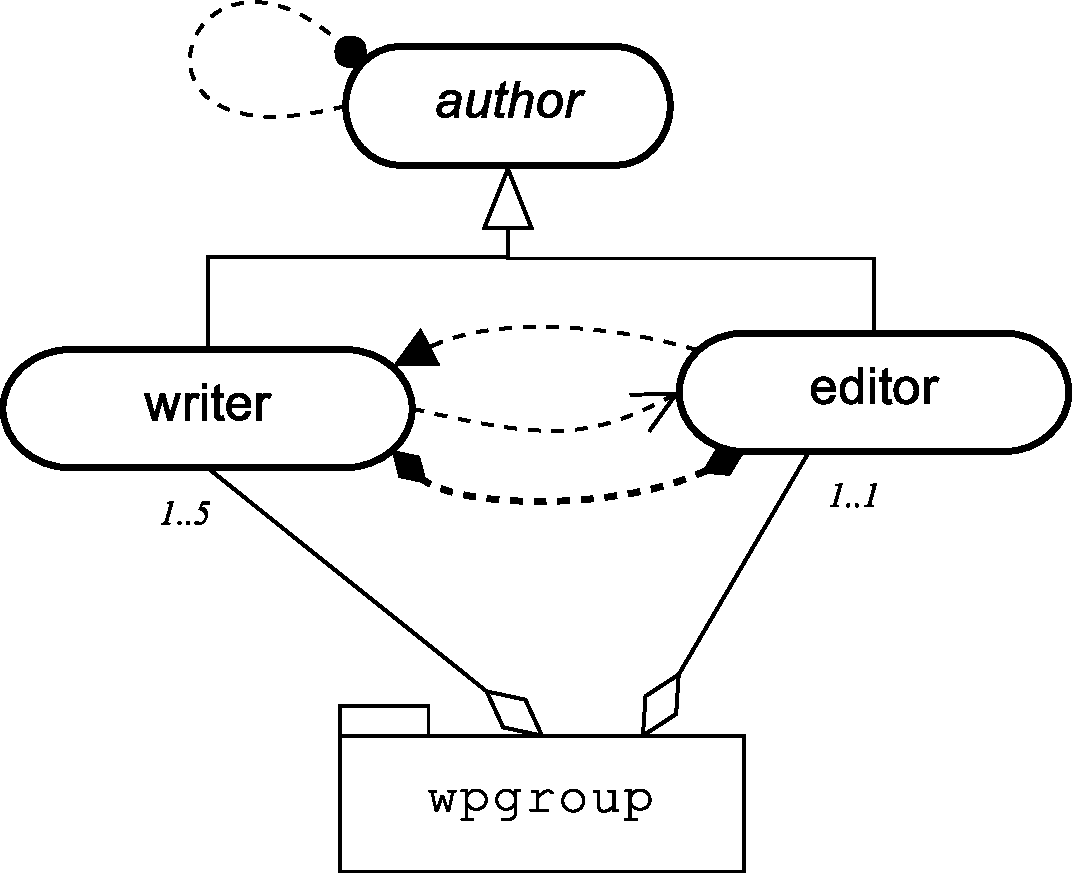
\includegraphics[width=.5\textwidth]{\pathwp/figures/writePaperSS}
\end{center}

\subsection{Functional Specification}

\begin{center}
  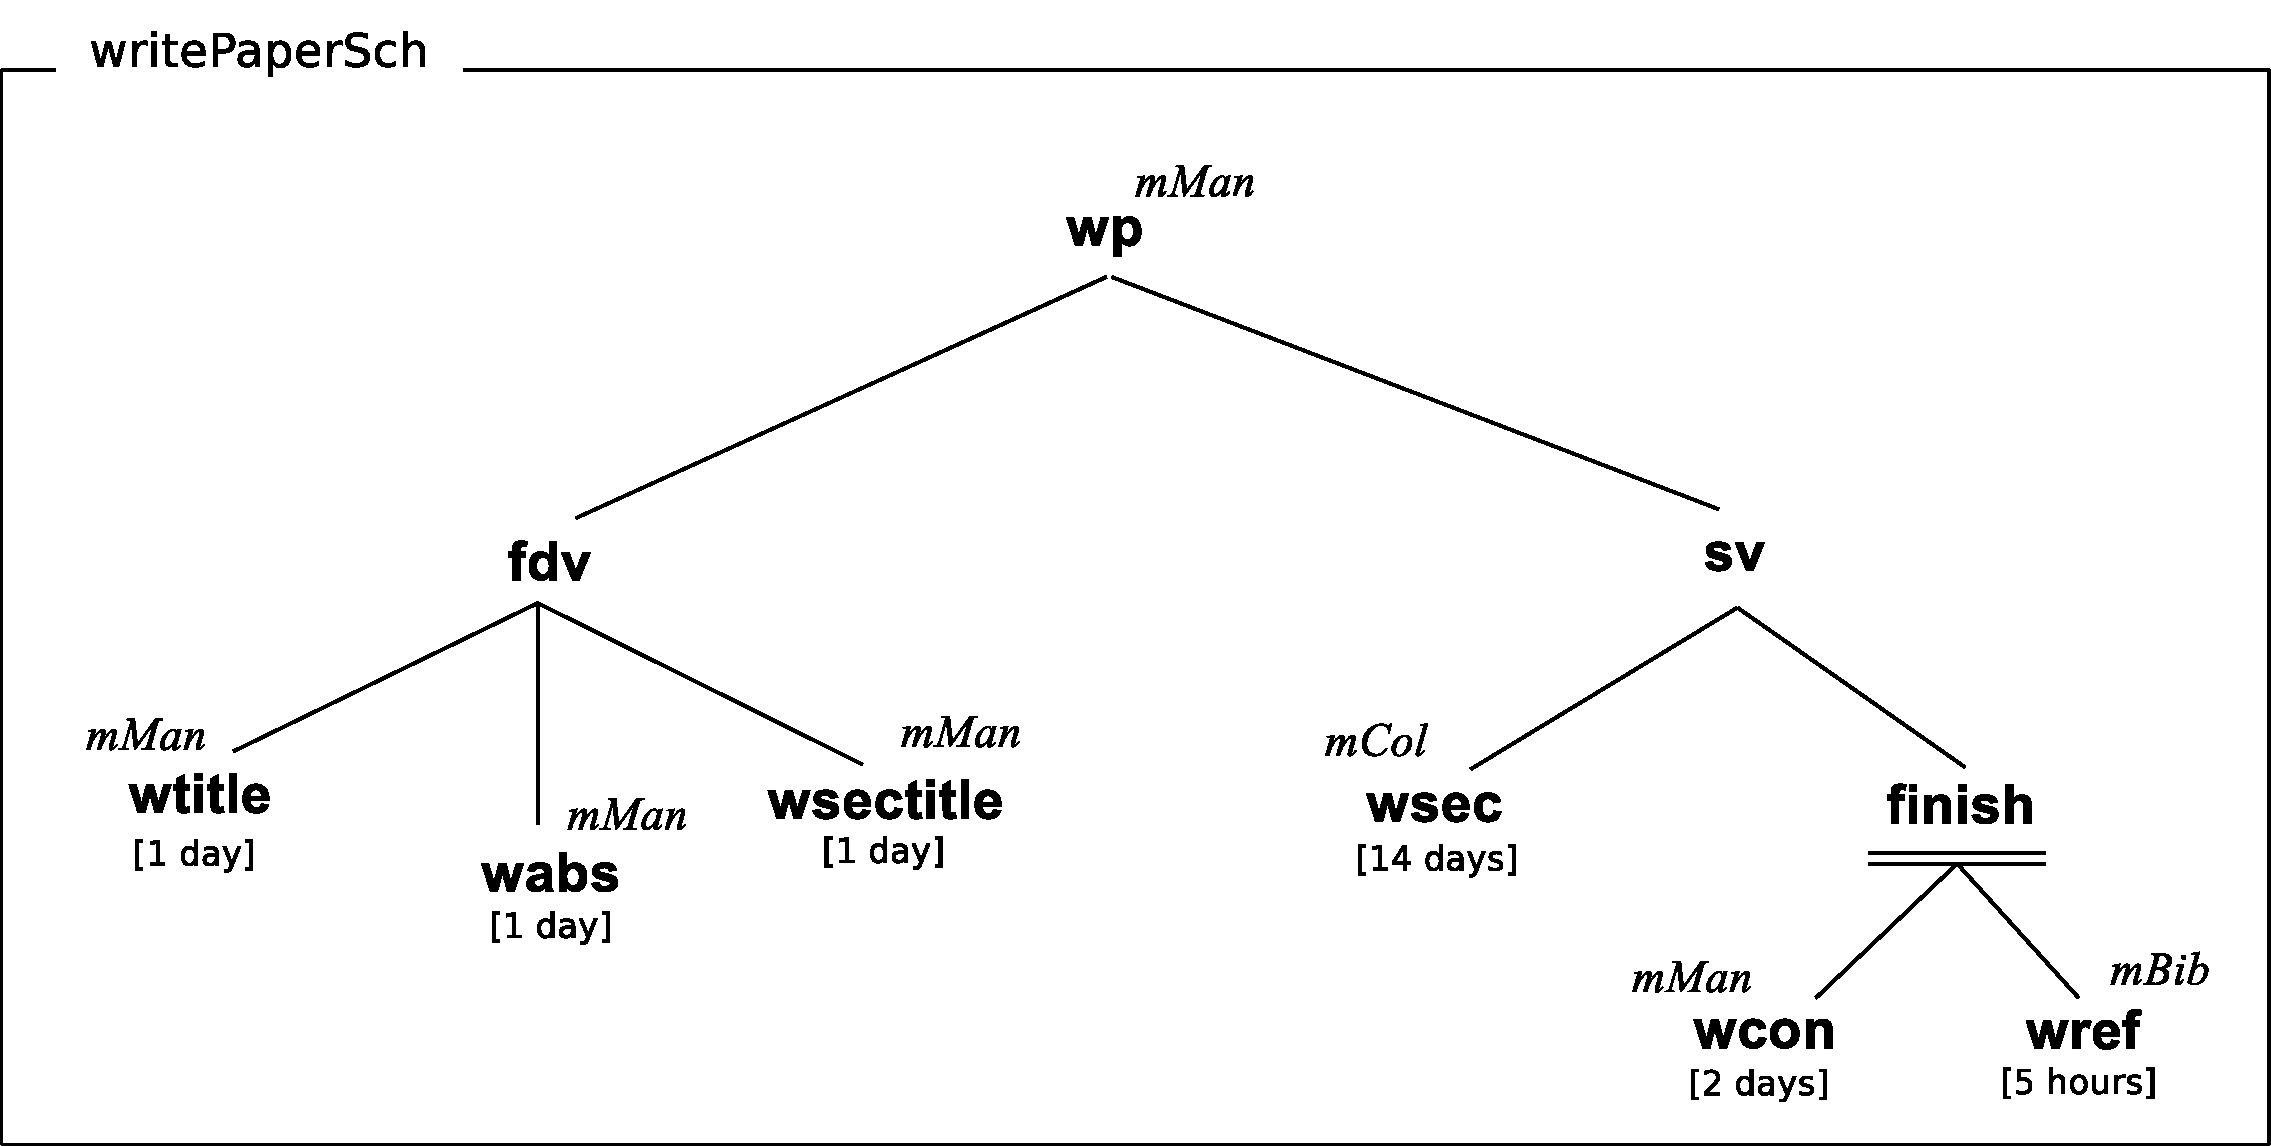
\includegraphics[width=\textwidth]{\pathwp/figures/writePaperFS}

  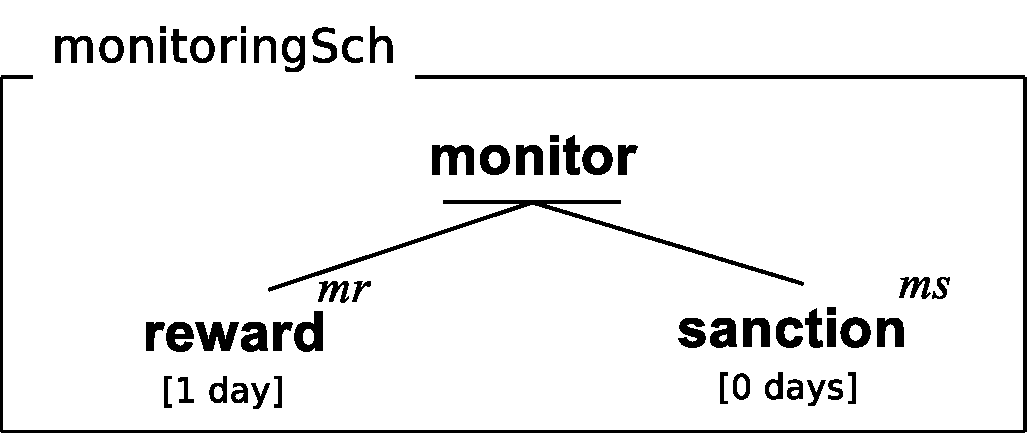
\includegraphics[width=.5\textwidth]{\pathwp/figures/monitoringFS}

  \newpage
  \textbf{Mission Cardinalities}

  \begin{tabular}{c c c c}
      \toprule
      mission & cardinality \\
      \midrule
      $mMan$ & 1..1 \\
      $mCol$ & 1..5 \\
      $mBib$ & 1..1 \\
      \midrule
      $mr$ & 1..1 \\
      $ms$ & 1..1 \\
     \bottomrule
   \end{tabular}

   \bigskip

   \textbf{Goals}

   \begin{tabular}{l c c c}
      \toprule
      goal & type & cardinality &  TTF \\
      \midrule
      \goal{wtitle} & achievement & 1 & 1 day\\
      \goal{wabs} & achievement & 1 & 1 day\\
      \goal{wsectitle} & achievement & all & 1 day\\
      \goal{wsec} & achievement & all & 7 days\\
      \goal{wcon} & achievement & 1 & 2 days\\
      \goal{wrefs} & achievement & all & 1 hour\\
      \midrule
      \goal{reward} & achievement & all & 0 day\\
      \goal{sanction} & achievement & all & 0 day\\
     \bottomrule
    \end{tabular}

\end{center}

\subsection{Normative Specification}

\begin{center}
   \begin{tabular}{l l c c c c c c}
      \toprule
      id & condition & role & type & mission & TTF \\
      \midrule
      n1 &  & editor  & permission & $mMan$ & -- \\
      n2 &  & writer  & obligation & $mCol$    & 1 day\\
      n3 &  & writer  & obligation & $mBib$    & 1 day\\
      n4 & unfulfilled(n2) & editor  & obligation & $ms$  & 3 hours\\
      n5 & fulfilled(n3)     & editor  & obligation & $mr$  & 3 hours\\
      n6 & \#goal\_non\_compliance & editor  & obligation & $ms$  & 3 hours\\
      n7 & \#role\_compatibility & editor  & obligation & $ms$  & 30 minutes\\
      n8 & \#mission\_cardinality & editor  & obligation & $ms$  & 1 hour\\
      \bottomrule
    \end{tabular}
\end{center}

\subsection{NOPL program}
{\small
\verbatiminput{\pathwp/wp-gen.npl}
}

\bibliographystyle{apalike}
\bibliography{jomi}

\end{document}
